\section{Introduktion till utvecklingsmiljön \coq Ide}

För närvarande finns det två olika utvecklingsmiljöer för \coq. Det är \coq Ide
som är en fristående utvecklingsmiljö och Proof General som är ett emacsläge.
Vi väljer att endast presentera \coq Ide då vårt projekt endast använder oss av
denna utvecklingsmiljö.

\subsection{Översikt av \coq Ide}

\coq Ide är en interaktiv utvecklingsmiljö där användaren kan formulera bevis
och skriva program samt att interaktivt bevisa dessa. I följande avsnitt
förklaras de viktigaste delarna med hjälp av skärmdumpar med exempelkod.

Figur~\ref{fig:oversikt} är en översikt av hela utvecklingsmiljön och dess
olika delar
\begin{enumerate}
\item Textredigerare. I den här rutan skriver användaren sina program och
  bevis. Den grönmarkerade (skuggade om du inte har färgskrivare) koden har
  tolkats av systemet.
\item Textfönster för mål och kontext. I bevisläge visas här vilka mål som ska
  uppnås och vilka hypoteser som för närvarande finns i kontexten. Dessa
  uppdateras efter varje utförd taktik.
\item Textfönster för meddelanden. Här dyker felmeddelanden, svar på
  gjorda sökningar och övrig information upp.
\item Knappar för att stega framåt eller bakåt i koden. När vi stegar framåt
  tolkas koden som stegas förbi av systemet.
\end{enumerate}

\filbreak

\begin{figure}[H]
  \centering
  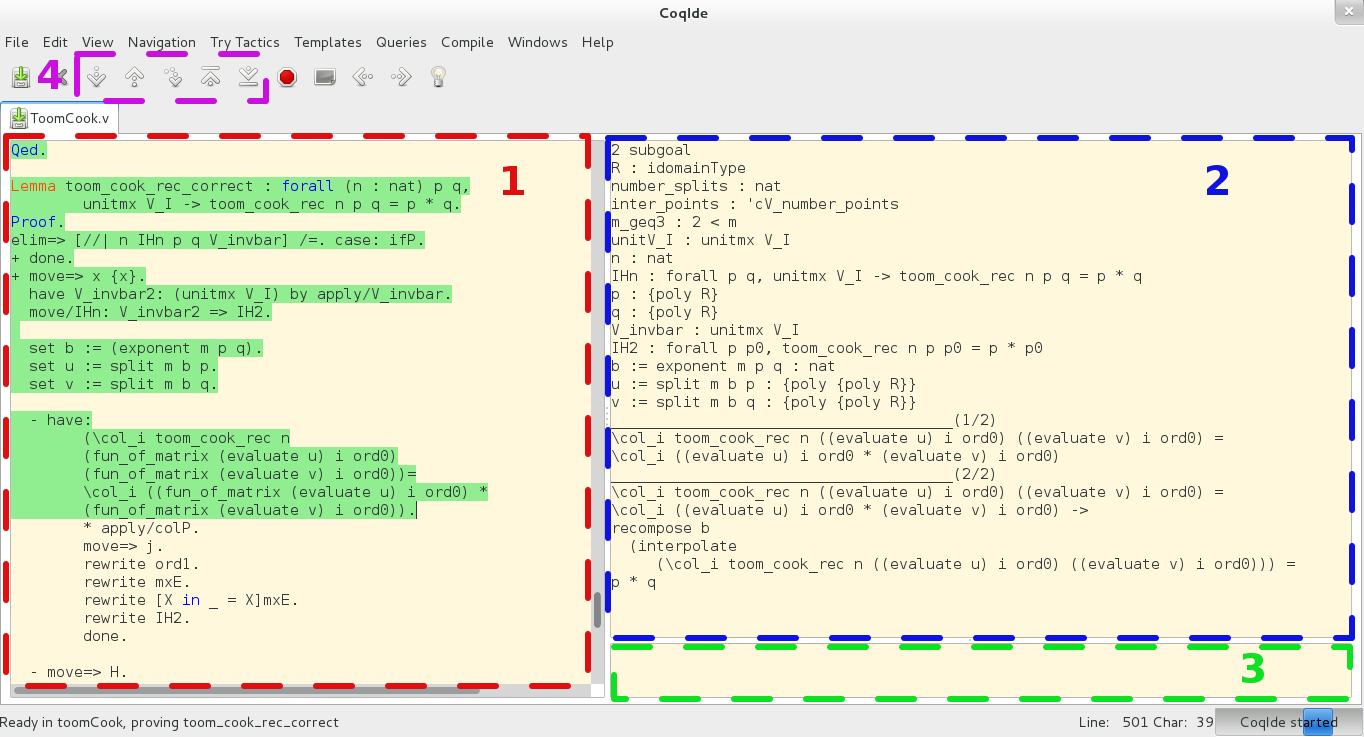
\includegraphics[width=\textwidth]{images/Overview}
  \caption[Översikt av \coq Ide]
   {Översikt av de olika delarna i \coq Ide}
  \label{fig:oversikt}
\end{figure}

Figur~\ref{fig:kontext} är är en förstoring av ruta 2 i Figur~\ref{fig:oversikt}
\begin{enumerate}
  \setcounter{enumi}{4}
\item Kontext, här visas vilka hypoteser och variabler som vi för tillfället
  har i beviset.
\item Mål, här visas vilka mål som ska uppnås. Det översta målet är det som
  användaren arbetar med för tillfället och det är det målet som kommer att
  påverkas av nästkommande taktik.
\end{enumerate}

\begin{figure}[H]
  \centering
  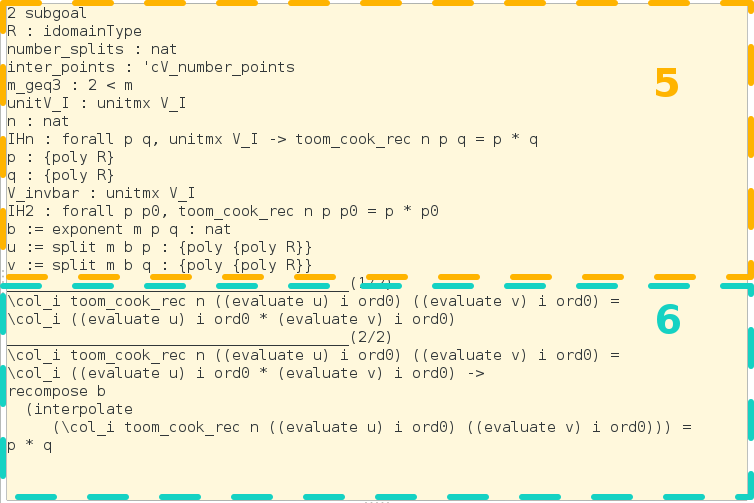
\includegraphics[width=150mm]{images/Kontext}
  \caption[Fönster för kontext och mål]
   {Textfönster för kontext och mål. Figuren visar en förstoring av ruta 2 i
    figur~\ref{fig:oversikt}}
  \label{fig:kontext}
\end{figure}

\subsection{Tolkning av kod}
Koden tolkas en sats i taget och de delar av koden som har blivit tolkade
markeras med en grön färg och det går inte längre att göra några ändringar i
dessa. Om man skulle vilja göra en ändring får man stega tillbaka i programmet
och göra ändringen. I följande sekvens av skärmdumpar visas några steg i ett
bevis.

Figur~\ref{fig:bevis1} visar ett exempel på ett bevis för att följande
påstående är en tautologi. En tautologi är en logisk sats som alltid är sant
oberoende av sanningsvärdena hos delsatserna.

\begin{figure}[H]
  \centering
  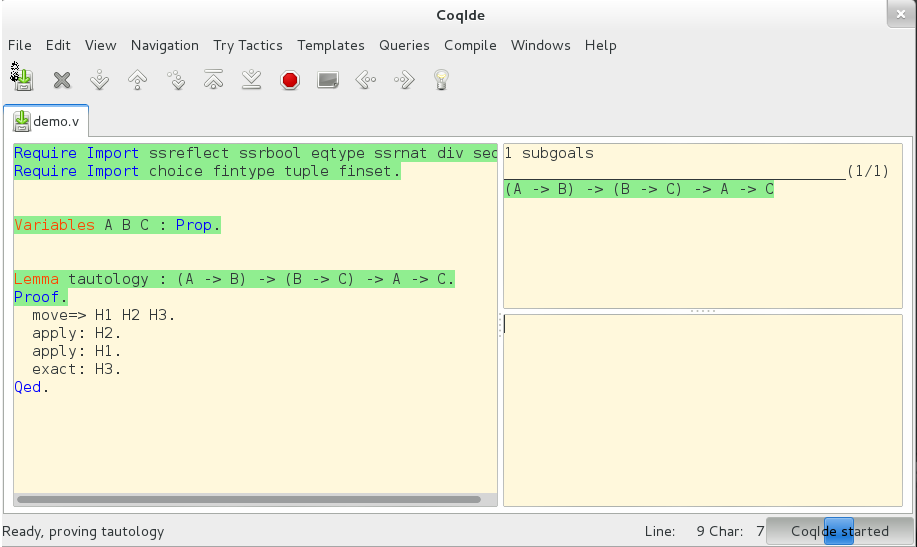
\includegraphics[width=100mm]{images/Proof_part1}
  \caption[Exempel på bevis i \coq{}]
   {Exempel på ett bevis för en tautologi i \coq{}}
  \label{fig:bevis1}
\end{figure}

Figurerna ~\ref{fig:bevis2} och ~\ref{fig:bevis3} visar den interaktiva biten
mellan \coq Ide och användaren. Notera hur mål och kontext uppdateras efter att
en taktik används och att den taktik som har tolkats blir grönmarkerad.

\begin{figure}[H]
  \centering
  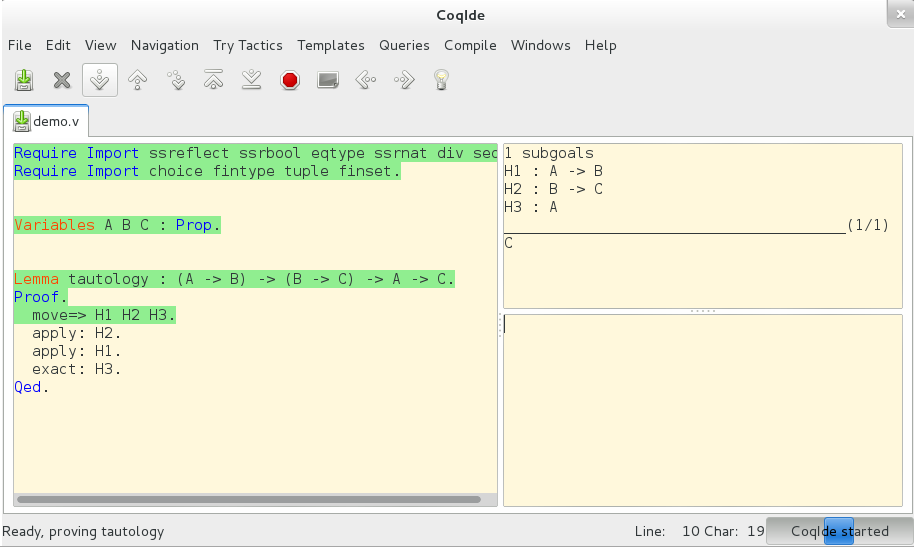
\includegraphics[width=150mm]{images/Proof_part2}
  \caption[Bevis i \coq Ide]
   {Vi har nu flyttat hypoteserna ($A \rightarrow B$), ($B \rightarrow C$) och $A$
    från målet till kontexten med taktiken \C{move}}
  \label{fig:bevis2}
\end{figure}

\begin{figure}[H]
  \centering
  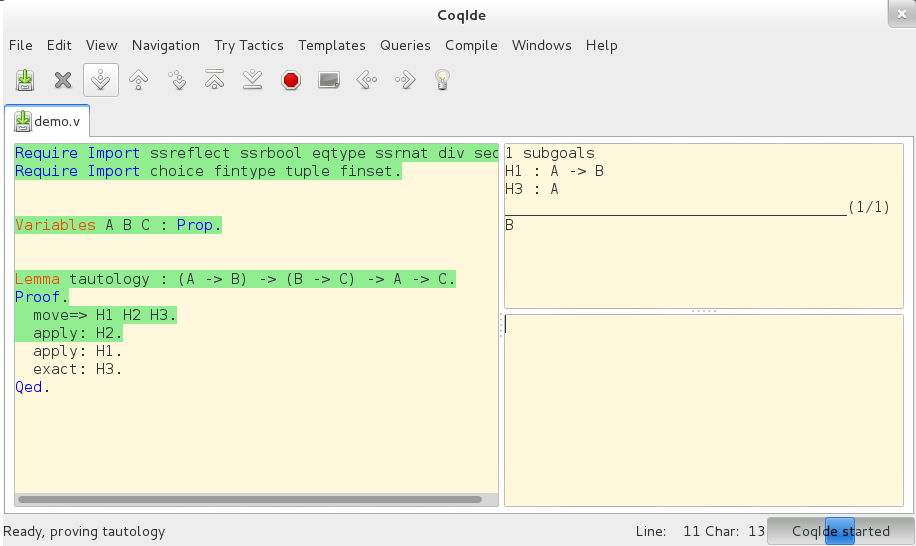
\includegraphics[width=150mm]{images/Proof_part3}
  \caption[Bevis i \coq Ide]
   {Vi har nu använt oss av hypotesen ($B \rightarrow C$) och vi
    kan se att målet nu har ändrat sig från $C$ till $B$}
  \label{fig:bevis3}
\end{figure}
